\section{C语言的数据基石——变量、常量和字面量}

\subsection{数据的原形：字面量(literal)的概念与初步认识}

首先来解释一下什么是字面量(\texttt{literal})。在C语言中，字面量(\texttt{literal})指的是
直接出现在源代码中的“数值”本身，无需标识符（名字）即可使用。说得
大白话一点，就是代码中一个又一个所见即所得的数据。
如\autoref{lst:literal_example}
所示，代码中出现的一个又一个常量数字如\texttt{42}、\texttt{'A'}、
\texttt{3.1416}、\texttt{Hi}
就是字面量(\texttt{literal})。


\begin{lstlisting}[language=C,caption={C 语言中字面量的示例},label={lst:literal_example}]
#include <stdio.h>

int main(void) {
    int x = 42;             // 42 是整型字面量
    char c = 'A';           // 'A' 是字符字面量
    double pi = 3.1416;     // 3.1416 是浮点字面量
    printf("%s\n", "Hi");   // "Hi" 是字符串字面量
    return 0;

  //注意我这里指的不是变量名 x、c、pi，而是等号右边的那些具体数值  
}
\end{lstlisting}

\textbf{在汇编层面，字面量并不占用数据内存空间RAM（字符串字面量除外）}，
通常情况下数值字面量并不会被放入 RAM(数据存储区)，
而是以 \textbf{立即数（Immediate Value）} 的形式
直接编码到机器指令中。例如此处指令中的字面量0x12：

\begin{lstlisting}
MOV A, #0x12       ; 汇编语言，将立即数 0x12 加载到累加器 A 中
\end{lstlisting}

该指令通常在机器码中被编码为：

\begin{lstlisting}
74 12     ; 机器码表示：74 是 MOV A 这一动作的指令代码, 12 是立即数部分
\end{lstlisting}

这里的立即数 \verb|12H| 是指令字节的一部分，
最终都会随着指令流一起储存于程序存储器（Flash/ROM）中，而非 RAM 数据区。

\subsubsection{补充：字面量的定义}
在 \textbf{C 语言标准}（如 ISO/IEC 9899:2018, C17）中，``字面量''（\textit{literal} 或 \textit{literal constant}）是一个正式存在的术语。  
它指的是 \textbf{直接出现在源代码中的常量值}，无需标识符即可使用。


\subsubsection{常见字面量的种类（根据 C17）}

\begin{center}
\begin{tabular}{lll}
\hline
\textbf{字面量类型} & \textbf{示例} & \textbf{说明} \\
\hline
整型字面量 (integer literal) & \verb|123|, \verb|0x7B|, \verb|010| & 十进制、十六进制、八进制整数 \\
浮点型字面量 (floating-point literal) & \verb|3.14|, \verb|1e-3| & 双精度浮点数 \\
字符字面量 (character constant) & \verb|'A'|, \verb|'\n'| & 单个字符，本质为 \verb|int| 类型 \\
字符串字面量 (string literal) & \verb|"Hello"| & 以 \verb|\0| 结尾的 \verb|char| 数组 \\
\hline
\end{tabular}
\end{center}

\textbf{枚举常量（enumeration constant）} 虽然是常量，但它是通过标识符声明的，不属于“字面量”。


\subsubsection{与“常量表达式”的区别}
\begin{itemize}
    \item 字面量是 \textbf{最简单的常量表达式（constant expression）}，但常量表达式可以包含运算符（如 \verb|2+3|），而 \verb|2+3| 不是字面量。
    \item 在 C 标准的语法描述中，字面量属于 \textbf{primary expression} 类别之一。
\end{itemize}

\subsubsection{与“宏”或“const 对象”的区别}
\begin{itemize}
    \item 宏替换发生在预处理阶段，宏展开后可能变成字面量，但宏名本身不是字面量。
    \item \verb|const int x = 5;| 中 \verb|x| 是标识符，不是字面量，虽然它可能在编译期有常量值。
\end{itemize}

这两部分属于“变量与常量”的范畴，后续章节会详细介绍。所以现在看不懂也没事，后续看到相关的
章节再回来复习此处内容即可。


\newpage


\subsection{字面量的进制与类型区分}
在前面的学习中，我们已经了解了字面量的基本概念。我们清楚了
字面量是没有标识符的常量数据，是直接写在代码中的数据本身。
但是有一点我们前面没有提及，那就是
字面量虽然没有独属于自己的标识符，但是它有自己的类型和进制。
那么在详细阐述字面量的类型与进制区分的相关知识之前，我们先回归到
我们最熟悉的场景——日常生活中的数字。


在我们日常生活中，我们每天都会接触大量的
数据，比如购物、计数。但我们从来不会纠结于
数据类型或是进制这些乱七八糟的东西。这是因为
在日常生活中，我们普遍使用\textbf{十进制}，同时我们思维
也是抽象地、没有物理内存限制的，也就不存在\textbf{数据类型}的问题
——我们讨论的就是纯粹的基于数学的数字概念。
所以对于我们彼此交流的时候，从来都不会纠结于进制、类型问题。

\begin{figure}[htbp]
  \centering
  
\includegraphics[width=0.7\linewidth]{figures/daily life.jpg}
  \caption{日常生活}
  \label{fig:daily life}
\end{figure}

\newpage
但在计算机中可不是这样，首先在计算机底部存储数字
使用二进制，而其他八进制、十六进制等进制也是常见的表示方式，
再加上由于计算机存储数据的方式不同又诞生了浮点数
、整型数、字符。

所以当你冷不丁地给计算机抛出一个数字42时,计算机
并不能理解这个数字到底是什么进制、类型，如下面这行
所示，计算机并不能理解这是十进制的42，还是
八进制的\texttt{34}，还是十六进制的\texttt{68}。它更无法理解这到底是
\texttt{int}、\texttt{double}还是\texttt{float}。

计算机此时只能按照默认处理规则进行处理，默认情况下这个\texttt{42}
将被理解为十进制、\texttt{int}类型的数据。但如果你的本意并不是这样，
而是想表达其他进制或类型的数据，那么计算机就会误解你的意思。那么在
工程场景下，往往就会引发严重的错误。


\begin{lstlisting}
                                      42          //你到底想表达什么呢？
\end{lstlisting}

计算机遇到这种情况时，
它是无法理解的，因为它不知道这个数字到底是什么进制、类型。
这就好像一个麻瓜突然看到一个魔法师念咒语一样（来自哈利波特），
它根本无法理解魔法师到底在说什么。对于这种情况，工程师经常形象地
戏称为魔法数字（Magic Number）。

\textbf{所以这里就引出了C语言对字面量的具体区分方式。——通过
“前缀（\texttt{prefix}）”和“后缀（\texttt{suffix}）”来对
字面量（\texttt{literal}）进行类型和进制的区分。}

C 语言里面通过“前缀（\texttt{prefix}）”和“后缀（\texttt{suffix}）”来对
字面量（\texttt{literal}）进行类型和进制的区分。
本节总结了 C 语言中通过前缀 \texttt{（Prefix）} 与
后缀 \texttt{（Suffix）} 来区分字面量的进制与类型的方式。
内容适用于 C89/C99/C11/C23 标准。


\subsubsection{整数：通过前缀区分进制}

整数字面量可使用前缀（\texttt{prefix}）确定进制，如 \autoref{tab:int-prefix} 所示。

\begin{table}[h!]
\centering
\caption{整数前缀及其含义}\label{tab:int-prefix}
\begin{tabular}{c|c|c}
\hline
前缀 & 进制 & 示例 \\ \hline
(无前缀) & 十进制 & \verb|123| \\
\verb|0| & 八进制 & \verb|0123| （十进制 83）\\
\verb|0x| / \verb|0X| & 十六进制 & \verb|0x123| （十进制 291）\\
\verb|0b| / \verb|0B|（C23） & 二进制 & \verb|0b1010| （十进制 10）\\
\hline
\end{tabular}
\end{table}


注意：
\begin{itemize}
    \item 以 \texttt{0} 开头的整数默认按八进制解析（如 \texttt{0123} $\neq$ \texttt{123}）。
    所以在 C 语言中避免使用前导零，以免引起歧义。这算是一个非常经典的错误原因呢。
    \item  C89/C99/C11 没有二进制前缀， 直到 C23 才正式加入\texttt{0b}作为二进制前缀，
    有些编译器（如 GCC）较早支持。
    \item C 语言中只有十六进制浮点数可以带前缀，其他进制的浮点数一律不允许带前缀。
    （具体见后文）。
\end{itemize}


 
\subsubsection{整数：通过后缀区分类型}



整数字面量的类型可由后缀（Suffix）确定。表 \ref{tab:int-suffix} 汇总了常见后缀。

\begin{table}[h]
\centering
\caption{整数类型后缀}\label{tab:int-suffix}
\begin{tabular}{cccc}
\hline
后缀 & 类型 & 示例 & 中文含义 \\ \hline
(无后缀) & int & \verb|123| & 整型（默认类型） \\

\verb|u| / \verb|U| & unsigned int & \verb|123U| & 无符号整型 \\

\verb|l| / \verb|L| & long int & \verb|123L| & 长整型 \\

\verb|lu| / \verb|LU| & unsigned long & \verb|123UL|, \verb|123LU| & 无符号长整型 \\

\verb|ll| / \verb|LL| & long long int & \verb|123LL| & 长长整型 \\

组合使用 & unsigned long long 等 & \verb|123ULL|, \verb|123LLU| & 无符号长长整型 \\ \hline
\end{tabular}
\end{table}



如\autoref{lst:int-suffix}所示，不同的类型其实意味着\textbf{存储空间}和\textbf{取值范围}
的不同。
所以当你由于不同的应用场景需要表示不同范围的整数时，
可以使用相应的后缀来指定类型。如果这个范围不匹配，
编译器会报错或发出警告。


\begin{lstlisting}[language=C,caption={后缀示例},label={lst:int-suffix}]

123        // int (默认类型)             -2147483648 ～ 2147483647 (32位系统)
123U       // unsigned int              0 ～ 4294967295

123L       // long int                  -2147483648 ～ 2147483647 (32位系统)
123LU      // unsigned long int         0 ～ 4294967295 (32位系统)

123LL      // long long int         -9223372036854775808 ～ 9223372036854775807
123LLU     // unsigned long long int    0 ～ 18446744073709551615

  
//以上给出的数据范围基于常见的32位和64位系统，
//实际范围基于编译器、CPU 架构和操作系统选择的数据模型而异。

\end{lstlisting}

\vspace{1em}
\noindent\textbf{注意}

作为整数字面量后缀：llu 和 ull 完全等价，可以随便使用，没有任何问题。
但在 printf 格式字符串中：必须用 \%llu，不能用 \%ull。所以我推荐大家统一
记忆llu。

\newpage



\subsubsection{浮点数：无前缀（Prefix 不可用）}%有假标题

浮点数\textbf{不能使用前缀} 来表示进制（十六进制除外），
不能像整数那样写成八进制、二进制形式：

\begin{itemize}
    \item \verb|012.3| （非法，浮点不能为八进制）
    \item \verb|0b1.01| （非法，C 不支持二进制小数）
    \item \verb|0x3.14| （非法的普通十六进制形式）
\end{itemize}



因此：浮点字面量不允许使用任何前缀。但凡事总有例外，在C语言中，十六进制浮点数就能表示
，但其他进制的浮点数一律不允许带前缀。也就是说
\[\textbf{C语言中浮点数字面量只能有两种存在方式，第一种是默认的十进制，第二种是十六进制。}\]

\paragraph{使用前缀表示十六进制浮点字面量（C99 及以后）}


从 C99 标准开始，C 语言\textbf{新增}了一类字面量：
\emph{十六进制浮点字面量}（hexadecimal floating constant）。  
这一类浮点字面量是允许使用 \verb|0x| 或 \verb|0X| 前缀的，
只是语法与整数常量不同，因此很多教材在入门阶段会直接略去不讲。

\vspace{1em}




\begin{enumerate}[label=(\arabic*), wide=0pt]
    \item 十六进制浮点常量的一般形式

\noindent{十六进制浮点常量的大致结构可以写成:}

\[
\begin{aligned}
  \underbrace{\mathtt{0x}\ \mbox{/}\ \mathtt{0X}}_{\mbox{十六进制前缀}}
  \quad
  \underbrace{\mbox{十六进制数字（可带小数点）}}_{\mbox{significand}}
  \quad
  \underbrace{\mathtt{p}\ \mbox{/}\ \mathtt{P} + \mbox{十进制指数}}_{\mbox{以 2 为底的指数}}
  \quad
  \underbrace{\mbox{浮点后缀 }(\mathtt{f},\mathtt{F},\mathtt{l},\mathtt{L})}_{\mbox{类型说明}}
\end{aligned}
  \]

更口语一点的记忆方式：  
\begin{center}
\verb|0x| \texttt{十六进制小数部分} \verb|p| \texttt{十进制整数指数} \texttt{[可选后缀]}
\end{center}

\noindent
其数值等价于：
\[
  \pm\,\mbox{(十六进制有效数字)} \times 2^{\mbox{指数}}
\]

\newpage

    \item 若干合法示例
    
\begin{table}[H]
\centering
\caption{十六进制浮点常量示例及其对应值}\label{tab:hex-float}
\begin{tabular}{ll}
\toprule
字面量 & 对应的十进制值（大致含义） \\
\midrule
\verb|0x1.2p3|       & $(1 + 2/16) \times 2^{3} = 1.125 \times 8 = 9.0$ \\
\verb|0x9A.8p-1|     & $(154 + 8/16) \times 2^{-1} = 154.5 / 2 = 77.25$ \\
\verb|0x1.921fb6p1f| & $\approx 3.1415927\quad(\texttt{float}，接近 \pi)$ \\
\bottomrule
\end{tabular}
\end{table}






下面用代码形式再演示一次（需要支持 C99 及以上标准的编译器，例如 \verb|gcc -std=c11|）：

\begin{lstlisting}[language=C,caption={十六进制浮点常量示例},label={code:hex-float}]
#include <stdio.h>

int main(void) {
    double b = 0x1.8p1;   // 3.0
    double c = 0x1.fp2;   // 7.75
    float  d = 0x.ap-3f;  // 0.078125f

    printf("b = %f\n", b);
    printf("c = %f\n", c);
    printf("d = %f\n", d);
    return 0;
}
\end{lstlisting}

\vspace{1em}




    \item 为什么 \texttt{0x3.14} 仍然是“非法写法”？
    

在上文我们给出例子：\verb|0x3.14| “非法的普通十六进制形式”。  
这个结论在 C99 之后\textbf{依然成立}，原因是：

\begin{itemize}
  \item 对整数常量来说，形如 \verb|0x3.14| 带小数点，本来就不是合法的“整数十六进制字面量”；
  \item 对十六进制浮点常量来说，\verb|0x3.14| 也\textbf{不完整}，因为缺少必须的 \verb|p| 或 \verb|P| 指数部分。
\end{itemize}

也就是说，\verb|0x3.14| 只是一个“十六进制有效数字”，\textbf{不是}完整的“十六进制浮点常量”。  
如果把它补写完整，例如：
\[
  \verb|0x3.14p0|,\quad
  \verb|0x3.14p+0|,\quad
  \verb|0x3.14p4|
\]
这些才是标准允许的、真正合法的十六进制浮点字面量。






    \item 浮点数十进制科学计数法的写法补充
    
刚才我们前面讨论了十六进制浮点数的写法，顺便补充一下
十进制浮点数的科学计数法写法，十进制浮点数
除了常见的 \verb|3.14| 形式外，还可以使用十进制的科学计数法
来表示浮点数，例如：

\begin{itemize}
    \item \verb|1.23e2|：代表 $1.23 \times 10^2 = 123.0$
    \item \verb|3.14E-2|：代表 $3.14 \times 10^{-2} = 0.0314$
\end{itemize}

其通用格式为：
\[
  \texttt{尾数部分} \quad \texttt{e/E} \quad \texttt{指数部分}
\]

其中：
\begin{itemize}
    \item \textbf{尾数部分(\texttt{Mantissa})}：可以是整数或小数（如 \verb|1.23| 或 \verb|3|）。
    \item \textbf{e/E}：作为分隔符，表示“乘以 10 的多少次方”。
    \item \textbf{指数部分(\texttt{Exponent})}：必须是\textbf{整数}（如 \verb|2|、\verb|-3|），不能是小数。
\end{itemize}

\textbf{非法示例}：
\begin{itemize}
    \item \verb|e3| （缺少尾数）
    \item \verb|2.1e| （缺少指数）
    \item \verb|2.1e3.5| （指数必须是整数）
\end{itemize}
\newpage


\subsection{浮点数的后缀}%有代码，有表格

浮点字面量只能用后缀确定类型，如表 \ref{tab:float-suffix} 所示。

\begin{table}[h]
\centering
\caption{浮点数字面量类型与后缀}\label{tab:float-suffix}
\begin{tabular}{cccccc}
\hline
后缀 & 类型 & 示例 & 字节数（典型） & 精度（有效数字） & 中文含义 \\ \hline

(无后缀) & double & \verb|3.14| 
& 8 字节
& 约 15–16 位 
& 双精度浮点数(默认) \\

\verb|f| / \verb|F| & float & \verb|3.14f| 
& 4 字节
& 约 6–7 位 
& 单精度浮点数 \\

\verb|l| / \verb|L| & long double & \verb|3.14L| 
& 10–16 字节
& 约 18–33 位 
& 扩展精度浮点数 \\

\hline
\end{tabular}
\end{table}


示例：



\begin{lstlisting}[language=C,caption={浮点数后缀示例},label={code:float-suffix}]
#include <stdio.h>

int main(void) {
3.14f        // float
2.718L       // long double
1e-3         // double（默认类型）
}
\end{lstlisting}


\subsection{前后缀小结}

\begin{itemize}
    \item 整数字面量：\textbf{前缀区分进制，后缀区分类型}。
    \item 浮点字面量：\textbf{无前缀，只能用后缀区分类型}。
    \item C99 起提供十六进制浮点字面量（如 \verb|0x1.2p3|）。
\end{itemize}



\end{enumerate}
\newpage


\subsection{字面量底层机制揭秘（ARM）}

要深入理解字面量在硬件层面的行为，我们需要先了解一些计算机体系结构的基础知识（注：本节内容涉及计算机组成原理，建议读者结合相关背景知识阅读）。

在嵌入式开发领域，ARM 架构占据了统治地位（本书所有示例均基于 ARM 架构）。经典的 ARM 指令集通常采用固定的 \textbf{32 位指令长度}。这意味着，每一条机器指令——无论是运算、跳转还是访存——都必须严格限制在 32 个二进制位（4 字节）之内。

这就引出了一个物理上的\textbf{根本矛盾}：

\begin{itemize}
    \item \textbf{指令容器的局限性}：一条指令只有 32 位。在这有限的空间内，CPU 必须编码操作码（Opcode）、目标寄存器、源寄存器等控制信息。留给嵌入“字面量数值”的空间往往非常有限（通常不足 12 位）。
    \item \textbf{数据数值的广度与复杂度}：一个标准的 32 位整数覆盖了 32 位全空间；而一个 IEEE 754 标准的浮点数，其编码结构更是复杂且同样占据 32 位或更多。
\end{itemize}

显然，我们无法将一个任意的 32 位大整数（例如 \texttt{0x12345678}）或者复杂的浮点数（例如 \texttt{3.14159}）直接“塞”进一条同样只有 32 位宽、且还需要包含操作码的指令中。

为了解决这个问题，ARM 架构设计了一套极具智慧的分级处理机制。
我们可以将它们形象地比喻为\textbf{“随身携带”}和
\textbf{“去仓库取”}两种模式。

\subsubsection{小整数：VIP 通道（塞进指令中，随身携带）}

\begin{enumerate}[label=(\arabic*), wide=0pt]
    \item \textbf{适配情况}：符合ARM指令规则(“8 位基数 + 偶数循环右移”)的字面量
    （例如 \texttt{0xFF}, \texttt{0x100}）。此时该小整数字面量由于
    值小简单（可以通过简单的移位操作构造出来），因此可以直接嵌入到指令内部。

    \item \textbf{底层机制}：立即数寻址 (Immediate Addressing)。
    \item \textbf{硬件过程}：
    
    
    \begin{enumerate}[label=\ding{\numexpr171+\arabic*}]
        \item 编码阶段 (Source): 你在代码中写下 \texttt{int a = 12;} 或汇编语句 \texttt{MOV R0, \#12}。
        
        \item 编译阶段 (Compile): 编译器识别出数值“12”符合立即数编码
        规则，将其拆分为 $Value$ (8位) 和 $Rotate$ (4位)，直接\textbf{硬编码}在 
        32 位机器指令内部。数据此时不再是独立的数据，而是指令的一部分。
        
        \item 链接阶段 (Link): 链接器根据链接脚本（Linker Script），
        为包含该指令的代码段 (.text) 分配未来的 \textbf{Flash 的特定地址}（提前建立一个映射关系\footnote{这里的映射其实是一个数学术语，
        简单理解其实就是函数中自变量x和应变量y的一一对应关系。
        对应到这里就是地址和指令在编译器的帮助下建立起了
        一一对应关系，但此时还未进行实际的地址分配，你可以理解为指令（里面包含着字面量数据）和物理地址提前订婚哈哈哈。}）。
        此时字面量数据并没有独立的地址，它寄生在指令的地址中，或者说它本就是指令的一部分。
        
        \item 烧录阶段 (Flash): 烧录器通过 JTAG/SWD 接口，
    按照上一步链接器生成的映射关系，
        将这条包含数据的指令二进制流写入单片机的 Flash 存储单元\footnote{
            这个时候你就可以理解为指令（里面包含着字面量数据）和物理地址实际结婚了，哈哈哈哈}。
        
        \item 硬件实体: 此时，数值在物理上表现为 Flash 中存储该指令的那
            几个晶体管的状态。CPU 取指时，数据随指令流直接进入 CPU，
        \textbf{无需额外的内存读取周期}。
    \end{enumerate}   
    
    
    编译器将数值拆分为 \textit{Value} (8位) 和 \textit{Rotate} (4位)，
    直接\textbf{硬编码}在 32 位指令内部。数据就在指令流中，随指令流一起存入ROM/Flash，无需占用额外的数据内存。
    \item \textbf{CPU 内部动作}：
    \begin{enumerate}[label=\ding{\numexpr171+\arabic*}]
        \item 取指解码后，8 位基数被送入 \textbf{桶形移位器 (Barrel Shifter)}。
        \item 移位操作在数据进入 ALU 之前由硬件并发完成。
        \item \textbf{耗时}：0 额外周期（极快）。
    \end{enumerate}
\end{enumerate}



\subsubsection{大整数与浮点数：物流通道（放到指定地点，去仓库取）}

\begin{enumerate}[label=(\arabic*), wide=0pt]
    \item \textbf{适配情况}：
    \begin{enumerate}[label=\ding{\numexpr171+\arabic*}]
        \item \textbf{大整数}：无法通过移位规则构造的 32 位整数（如 \texttt{0x12345678}）。
        \item \textbf{浮点数}：\textbf{几乎所有}浮点字面量（如 \texttt{3.14}）。由于浮点编码过于复杂，
        占据的位数过多，无法像整数那样压缩到指令中。
    \end{enumerate}





    \item \textbf{底层机制}：文字池 \footnote{注： 在较新
    的 ARM 架构（如 Cortex-M 使用的 Thumb-2 指令集）中，
    引入了 MOVW (加载低16位) 和 MOVT (加载高16位) 指令。
    这意味着现在的 CPU 也可以通过两条指令直接把一个 32 位
    大整数“拼”进寄存器，而不一定非要查文字池。但在经典 ARM 教
    学和底层原理理解中，“文字池”依然是最核心
    的概念。}(Literal Pool) + PC 相对寻址。



    \item \textbf{硬件过程}： 
    



 \begin{enumerate}[label=\ding{\numexpr171+\arabic*}]
    \item 编码阶段 (Source): 你在代码中写下大数 \texttt{int a = 0x12345678;} 或浮点数 \texttt{float f = 3.14;}。
    
    \item 编译阶段 (Compile):编译器发现这些数据太“笨重”，无法塞进一条指令，于是将它们从逻辑中剥离，统一收集放到代码段末尾的\textbf{文字池 (Literal Pool)} 中。同时，在原位置生成一条内存加载指令（整数用 \texttt{LDR}，浮点数用 \texttt{VLDR}），利用 \textbf{PC 相对寻址}指向该数据。
    
    \item 链接阶段 (Link): 链接器计算出加载指令与文字池中具体数据之间的\textbf{偏移量 (Offset)}，确保 $PC + Offset$ 能精确指向存放该数据的物理地址。
    
    \item 烧录阶段 (Flash): 烧录器将“加载指令”和“数据本身”分别写入 Flash 的不同位置。指令在前面的代码区，数据在后面的文字池区。
    
    \item 硬件实体: 此时，数据物理上存在于 Flash 的某个存储单元中。CPU 执行到该行代码时，必须发起一次对 Flash 的\textbf{读操作}，将数据从文字池搬运到寄存器中。
\end{enumerate}




    \item \textbf{CPU 内部动作}：
    \begin{enumerate}[label=\ding{\numexpr171+\arabic*}]
        \item CPU 计算 \texttt{PC + 偏移量} 获得文字池地址。
        \item 发起内存读操作，将数据搬运到通用寄存器 (R0-R15) 或浮点寄存器 (S0-S31)。
    \end{enumerate}
    大整数和浮点数字面量这样操作会比小整数耗时，
    因为涉及到内存访问，会比立即数慢（通常多 1-2 个周期）。
\end{enumerate}


\subsection{特殊字面量：字符串字面量 (String Literals) 底层机制解密}

在此前的学习中，我们建立了“小整数（VIP随身携带）”和
“大整数（去仓库取）”的思维模型。字符串字面量
（如 \texttt{"Hello"}）由于其体量巨大，
属于\textbf{最极端的“仓库存储”模式}。


\subsubsection{ 核心矛盾：因为字符串“太大”，只能“匿名”}

\begin{itemize}
    \item \textbf{指令容器的局限性}：一条 ARM 指令只有 32 位。
    \item \textbf{数据的庞大性}：即便是短字符串 \texttt{"Hello"} 
    也占据 48 位（6字节），远超寄存器(32位)和指令的承载能力。
    \item \textbf{结论}：字符串绝无可能进入 CPU 指令内部，
    它必须完全依赖外部存储空间，并通过\textbf{地址}进行访问，和大整数有些类似。
\end{itemize}


\subsubsection{ 从代码到晶体管：物理映射流程}

这是一个从软件定义到硬件实体的全过程：

\begin{enumerate}[label=(\arabic*), wide=0pt]
    \item \textbf{编码阶段 (Source)}: 
    你在代码中写下 \texttt{const char* p = "Hello";}。
    
    \item \textbf{编译阶段 (Compile)}: 
    编译器将 \texttt{"Hello"} 的数据（'H', 'e'...）归类为 \textbf{.rodata 段}。
    
    \item \textbf{链接阶段 (Link)}: 
    链接器查看链接脚本（.ld文件），决定 \texttt{.rodata} 
    段对应芯片的 \textbf{Flash 地址}（例如 \texttt{0x0800 1000}，与前文一样，此时只是提前
    建立映射关系）。
    
    \item \textbf{烧录阶段 (Flash)}: 
    烧录器通过 JTAG/SWD 接口，将数据真正写入单片机对应的 Flash 存储单元中。
    
    \item \textbf{硬件实体}: 
    此时，字符串物理上存在于 Flash 芯片内部，
    如果不进行擦除操作，掉电后依然存在。
\end{enumerate}


\subsection{核心疑问解答}

\subsubsection{Q1:CPU读取字符串地址的指令在哪里？和大整数一样吗？}

\textbf{答案：是的，机制非常相似，但多了一层“跳板”。}

\vspace{1em}

这正是 ARM 架构处理 32 位常量的标准做法。因为一条指令（32位）里
塞不下 32 位的地址（例如 \texttt{0x08001000}），所以
必须使用 \textbf{文字池 (Literal Pool)} 技术，而字符串和
大整数的区别在于，他们存放在文字池里的内容不同。字符串是地址，而
大整数是数值本身。

\begin{itemize}
    \item \textbf{位置}：读取地址的指令（通常是 \texttt{LDR}）确实写在前面的指令流中（代码段 .text）。
    \item \textbf{区别}：
    \begin{itemize}
        \item \textbf{大整数 (0x12345678)}：文字池里存放的直接是 \textbf{那个整数的值}。
        \item \textbf{字符串 ("Hello")}：文字池里存放的是字符串在 Flash 中的 \textbf{首地址（指针）}。
    \end{itemize}
\end{itemize}

\textbf{字符串字面量的执行三步走演示：}

\begin{enumerate}[label=\ding{\numexpr171+\arabic*}]
    \item \textbf{第一步（指令流中）}：
    CPU 执行 \texttt{LDR R0, [PC, \#offset]}。意思是：“去当前指令附近（文字池）帮我取个东西”。
    
    \item \textbf{第二步（文字池中）}：
    CPU 在文字池里找到了一个 32 位的数据，这个数
    据是 \texttt{0x0800 1000}（即字符串在 Flash 里的地址）。
    \textit{注意：这里只是拿到了钥匙，还没见到字符串。}
    
    \item \textbf{第三步（访问 .rodata）}：
    把刚刚找到的地址 \texttt{0x0800 1000} 装到 R0 寄存器里。
    后续指令使用 R0 寄存器里的地址（\texttt{0x0800 1000}）
    去访问 Flash，最终读出字符 \texttt{'H'}, \texttt{'e'},
     \texttt{'l'}, \texttt{'l'}, \texttt{'o'}，\texttt{'\textbackslash 0'}，
    合成一个字符串。
\end{enumerate}
\newpage

\subsubsection{Q2: 编译器把源代码分为几个区域？都映射到 Flash 吗？}

\textbf{答案：主要分为 4 个核心段。并非所有都映射到 Flash。}
\vspace{1em}

在嵌入式开发中，内存布局（Memory Layout）通常如下表所示：

\begin{table}[h]
\centering
\caption{常见的内存段分布}\label{tab:memory-sections}
\begin{tabular}{|l|l|l|l|}
\hline
\textbf{段名 (Section)} & \textbf{存放内容} & \textbf{Flash (ROM)} & \textbf{RAM (内存)} \\ \hline
\textbf{.text} & 代码指令、小整数 & \textbf{是 (存储地)} & 否 (XIP模式下) \\ \hline
\textbf{.rodata} & \textbf{字符串字面量}、const 常量 & \textbf{是 (存储地)} & 否 (直接读取) \\ \hline
\textbf{.data} & 已初始化的全局变量 & \textbf{是 (存初值)} & \textbf{是 (运行时)} \\ \hline
\textbf{.bss} & 未初始化的全局变量 & \textbf{否} & \textbf{是 (零初始化)} \\ \hline
\end{tabular}
\end{table}


\textbf{详细解析：}
\begin{itemize}
    \item \textbf{.text 和 .rodata}：这就是纯粹的“不动产”，一直躺在 Flash 里，CPU 直接去 Flash 里取指和读数据。
    \item \textbf{.data (特殊)}：比如 \texttt{int count = 10;}。这个 \texttt{10} 必须存在 Flash 里（否则掉电就没了），但程序运行时你需要修改变量，所以启动代码（Startup Code）会负责把这个 \texttt{10} 从 Flash \textbf{搬运} 到 RAM 中。
    \item \textbf{.bss}：比如 \texttt{int buffer[100];}。不需要在 Flash 占空间，启动时直接在 RAM 里清零即可。
\end{itemize}


\subsubsection{Q3: 字符串字面量在内存中具体是如何存储和处理的？}

\textbf{答案：它具有三个核心特性——只读存储、独立地址、类型退化。}

\begin{enumerate}[label=\ding{\numexpr171+\arabic*}]
    \item \textbf{存储位置：.rodata (只读数据段)}

    \textbf{定位}：通常存放在 \texttt{.rodata} (Read-Only Data) 段。

    \textbf{硬件映射}：在嵌入式系统（如 STM32）中，这一段直接映射在 \textbf{Flash (ROM)} 中。
    
    \textbf{后果}：这意味着它是硬件级别的“只读”。如果你试图通过指针修改它（如 \texttt{p[0] = 'X';}），会导致硬件错误（Hard Fault）。

    \item \textbf{内存占用：独立线性地址空间}

    每一个字符串字面量都在内存中拥有唯一的、独立的“门牌号”（线性地址）。
    哪怕是两个相同的 \texttt{"Hello"}，在某些编译器设置下也可能合并，但它们依然必须占据独立的地址空间，而不能像立即数那样“融化”在指令里。
\newpage
    \item \textbf{退化行为 (Decay)}

    \textbf{机制}：为了解决“搬运成本高”的问题，在表达式中，数组名自动转化为指向首元素的指针。
    \textbf{本质}：字符串字面量 \texttt{"Hello"} 的类型实际上是 \texttt{char[6]}（包含结尾的 \texttt{\textbackslash 0}）。
        
        \textbf{退化 (Decay)}：在 C 语言中，除了 \texttt{sizeof} 和 \texttt{\&} 操作符外，数组名在表达式中会自动转换为指向其第一个元素的指针。
    
    \textbf{类型变化}：
    \[ \text{源码形式：} \texttt{char[6]} \xrightarrow{\text{使用时}} \text{实际类型：} \texttt{char*} \]
    \textbf{CPU 视角}：CPU 处理的不是一串字符，而是一个 32 位的地址值（指针）。
\end{enumerate}


\newpage




\subsubsection{Q4: 如果 CPU 不小心“执行”到了 Literal Pool 里的数据会发生什么？}

\textbf{答案：CPU 会尝试将数据当作指令解码，通常导致“未定义指令异常”。}

\vspace{1em}

这是一个非常危险的情况。CPU 是一种 \textbf{取指-解码-执行} 的机器，它本身无法区分当前 PC 指向的是代码还是数据。如果程序逻辑出错（例如忘记写 \texttt{B} 跳转指令），导致 PC 滑入 Literal Pool：
\begin{itemize}
    \item 运气好时：数据对应的二进制位不符合任何有效指令格式，CPU 抛出 \textbf{Undefined Instruction Exception}，程序崩溃但能定位错误。
    \item 运气差时：数据恰好对应一条有效指令（例如 \texttt{AND} 或 \texttt{MOV}），CPU 会错误地执行它，破坏寄存器状态，导致难以调试的逻辑 Bug。
\end{itemize}
这也解释了为什么汇编器通常把 Literal Pool 放在 \textbf{无条件跳转指令} 之后。


\subsubsection{Q5: 既然要分散放置，编译器报错 "Literal pool out of range" 是什么意思？}

\textbf{答案：这意味着两个“文字池”之间的距离太远了，超过了指令的“射程”。}

\vspace{1em}

这直接对应了我们在上文中提到的 \textbf{PC 相对寻址限制}。
\begin{itemize}
    \item 假设你写了一个巨大的函数，长度超过了 4KB（在某些 ARM 模式下）。
    \item 这里的指令试图读取函数末尾 Literal Pool 里的常量。
    \item 但是指令中的 offset 字段位宽不够，无法编码这么大的距离。
\end{itemize}
此时必须在代码中间（例如循环或分支的跳转点之后）手动插入一个新的 \texttt{.ltorg}，强行在此处建立一个中转站（新的文字池），缩短指令到数据的距离。

\subsubsection{Q4: 为什么不直接把所有常量都放在 .data 或 .rodata 段，像普通全局变量那样访问？}

\textbf{答案：为了性能和代码密度。}

\vspace{1em}

虽然可以这样做，但并不高效：
\begin{itemize}
    \item \textbf{访问成本：} 访问 \texttt{.data} 段通常需要先加载数据段的基地址到寄存器，再进行偏移访问，这需要多条指令。
    \item \textbf{文字池优势：} 使用 Literal Pool 配合 \texttt{LDR}（PC 相对寻址），通常只需要 \textbf{一条指令} 就能把常量加载进寄存器，且不需要占用额外的寄存器来保存基地址。
\end{itemize}
Literal Pool 是为了解决“如何快速将大立即数加载到寄存器”这一具体微架构问题而生的特殊机制。




















\subsection{字面量底层硬件原理总结：三种字面量的“物流通道”}

我们可以用“物流运输”来形象地理解 CPU 处理这三种字面量的不同方式：

\begin{quote}
\textbf{核心逻辑}：能随身携带的（小整数）就随身带；带不动的（大整数）就放车厢（文字池）里查表；太占地方的（字符串）就只拿个提货单（地址），去仓库（.rodata）里取。
\end{quote}

\subsubsection{小整数：VIP 随身通道 (Immediate)}
\begin{itemize}
    \item \textbf{机制}：数值直接嵌入在指令代码中（如 \texttt{MOV R0, \#12}）。
    \item \textbf{特点}：\textbf{速度最快}。CPU 取指时，数据就跟着指令一起进来了，不需要额外的内存访问。
    \item \textbf{限制}：受指令长度限制，只能存很小的数（如 ARM 的 12 位编码）。
\end{itemize}

\subsubsection{大整数：专用物流通道 (Literal Pool)}
\begin{itemize}
    \item \textbf{机制}：数值太大塞不进指令，编译器把它存放在代码段末尾的“文字池”里。
    \item \textbf{特点}：\textbf{查表读取}。指令中存放的是“偏移量”，CPU 执行时通过 \texttt{LDR R0, [PC, \#offset]} 去文字池里把数搬运到寄存器。
    \item \textbf{代价}：多一次内存访问。
\end{itemize}

\subsubsection{字符串：超大集装箱 (Reference/Pointer)}
\begin{itemize}
    \item \textbf{机制}：字符串太长，只能存放在独立的 \texttt{.rodata} 段（仓库）。
    \item \textbf{特点}：\textbf{传递地址}。文字池里存的不再是数据本身，而是字符串在仓库里的\textbf{首地址}。
    \item \textbf{流程}：CPU 先去文字池拿地址（钥匙），再用地址去 \texttt{.rodata} 读数据（取货）。这是最慢的，涉及多次访存。
\end{itemize}






\begin{table}[h]
\centering
\caption{三种字面量底层机制对比}\label{tab:literal-mechanism-compare}
\begin{tabular}{|l|l|l|l|}
\hline
\textbf{维度} & \textbf{小整数 (VIP通道)} & \textbf{大整数 (物流通道)} & \textbf{字符串 (超大集装箱)} \\ \hline
\textbf{典型例子} & \texttt{MOV R0, \#0xFF} & \texttt{LDR R0, [PC, \#4]} & \texttt{const char* p = "Hi"} \\ \hline
\textbf{数据大小} & 极小 ($<12$ 位) & 标准 (32 位) & \textbf{不定长 (通常很大)} \\ \hline
\textbf{存储位置} & \textbf{指令内部} (代码段) & \textbf{文字池} (代码段末尾) & \textbf{.rodata} (独立数据段) \\ \hline
\textbf{获取方式} & 随身携带 (Immediate) & 查表读取数值 & \textbf{获取地址 (指针)} \\ \hline
\textbf{C语言表现} & \texttt{int} & \texttt{int} & \textbf{退化为 \texttt{char*}} \\ \hline
\end{tabular}
\end{table}

































\subsection{4. 关键思考：指针 vs 数组}

基于上述底层机制，理解以下两行代码的本质区别：

\begin{enumerate}
    \item \texttt{char *str = "Hello";} 
    \begin{itemize}
        \item \textbf{含义}：手里拿着一把仓库的\textbf{钥匙}。
        \item \textbf{操作}：\texttt{str} 变量直接指向 Flash 中的 \texttt{.rodata} 区域。
    \end{itemize}
    
    \item \texttt{char arr[] = "Hello";}
    \begin{itemize}
        \item \textbf{含义}：把仓库的货\textbf{搬运}一份到自家客厅。
        \item \textbf{操作}：CPU 执行一段搬运指令，将 Flash 中的字符串\textbf{复制}到 RAM (栈) 中。
    \end{itemize}
\end{enumerate}










\subsection{字符串字面量：只读段与栈拷贝 (String Literals)}

字符串字面量本质是匿名数组，但其存储和生命周期完全取决于\textbf{引用方式}。这是 C 语言中最大的内存陷阱之一。

\textbf{1. 指针引用} (\texttt{const char *p = "ABC";})

    存储位置 (Storage Location)

    \begin{itemize}
        \item \textbf{实体位置}：字符串常量直接存放在 \textbf{Flash (.rodata)} 段。
        \item \textbf{变量本质}：\texttt{p} 只是一个保存了 Flash 地址的指针变量。
    \end{itemize}

    性能与风险 (Performance \& Risk)

    \begin{itemize}
        \item \textbf{零拷贝}：没有数据搬运开销，直接读取 Flash。
        \item \textbf{只读陷阱}：试图修改 \texttt{p[0]} 会触发硬件错误 (HardFault)，因为 Flash 物理不可写。
    \end{itemize}

\textbf{2. 数组初始化} (\texttt{char arr[] = "ABC";})

    存储位置 (Storage Location)

    \begin{itemize}
        \item \textbf{源数据}：字符串实体依然存储在 Flash 中作为初始值。
        \item \textbf{运行时副本}：在函数执行时，数据会被\textbf{拷贝}到 \textbf{RAM (Stack)} 中。
    \end{itemize}

    性能特征 (Performance)

    \begin{itemize}
        \item \textbf{初始化开销}：编译器会生成 \texttt{memcpy} 或 \texttt{LDR/STR} 指令序列，在栈上复制一份副本。
        \item \textbf{RAM 消耗}：占用栈空间（字符串长度 + 1 字节）。
        \item \textbf{可修改性}：内容在 RAM 中，可以自由修改。
    \end{itemize}

\subsection{C99 复合字面量 (Compound Literals)}

\begin{itemize}
    \item \textbf{定义}：如 \texttt{(struct Point)\{.x=1, .y=2\}}，常用于结构体传参。
    \item \textbf{存储位置}：
    \begin{itemize}
        \item 若在函数内部使用，它是\textbf{自动变量}，存储在 \textbf{Stack (RAM)} 中。
        \item 每次进入作用域都会重新初始化（即从 Flash 搬运数据到 RAM）。
    \end{itemize}
    \item \textbf{注意}：如果不加 \texttt{const} 修饰，它们默认是可变的，且占用宝贵的栈空间。
\end{itemize}

\subsection{总结：字面量存储开销对比表}

\begin{center}
\begin{tabular}{|l|l|l|l|}
\hline
\textbf{字面量类型} & \textbf{物理存储 (Entity)} & \textbf{RAM 占用} & \textbf{CPU 访问方式} \\ \hline
小整数 (Immediate) & 指令流 (Flash) & \textbf{无} & 随指令流水线直接解吗 \\ \hline
大整数/浮点 (Pool) & 文字池 (Flash) & \textbf{无} & PC 相对寻址 (LDR) \\ \hline
字符串 (指针) & .rodata (Flash) & 仅指针变量 (4B) & 慢 (访问 Flash 总线) \\ \hline
字符串 (数组) & Flash $\rightarrow$ Stack & \textbf{有} (长度+1) & 快 (访问 RAM) \\ \hline
\end{tabular}
\end{center}



\subsection{3.~例外情况：字符串与大型常量表}
字符串字面量、查表数据、数组与较大的常数无法作为立即数编码。
编译器或汇编器会为它们分配独立的数据区（通常在 \texttt{.rodata} 或代码区的常量段）。
例如：
\begin{verbatim}
char s[] = "HELLO";
\end{verbatim}
会生成类似的数据块：
\begin{verbatim}
48 45 4C 4C 4F 00
\end{verbatim}

\subsection{4.~立即数大小受体系结构限制}
立即数字面量可编码的位数有限。例如在 8051：
\begin{itemize}
    \item \verb|MOV A, #imm8| 只允许 8 位立即数；
    \item \verb|MOV DPTR, #imm16| 支持 16 位立即数；
    \item 更大的常量无法使用立即数，需要放入程序存储器并通过 \verb|MOVC| 等指令访问。
\end{itemize}
例如：
\begin{verbatim}
MOV A, #0x1234   ; 不合法
\end{verbatim}
必须写为：
\begin{verbatim}
MOV DPTR, #TABLE
MOVC A, @A+DPTR
\end{verbatim}

\subsection{5.~字面量属于编译期常量}
字面量均在编译期确定，不需运行时求值。
因此它们不会在运行时消耗额外的 RAM 或寄存器资源。

\subsection{6.~更严谨的总结合述}
\begin{quote}
数值字面量通常以立即数形式直接编码到指令中，不占用 RAM 数据存储区。
这些立即数属于程序存储器的指令字节，而非独立数据块。
当字面量无法作为立即数表示（如字符串、数组、查表数据等），编译器将其存储在
程序存储器的数据段中，并通过指针或取数指令访问。
\end{quote}






但是字面量虽然没有独属于自己的标识符，但是它有自己的类型










% 在我们日常生活中，我们每天都会接触大量的
% 数据，比如购物、计数。但我们从来不会纠结于
% 数据类型或是字面量这些乱七八糟的东西。这是因为
% 在日常生活中，我们普遍使用\textbf{十进制}，
% 所以对于我们彼此交流的时候，从来都不会纠结于进制、类型问题。























单纯的“变量”在嵌入式里是不够用的，我们还需要给它贴标签，告诉编译器如何对待它。
我们知道，诸如数字、文字、符号、图形、音频、视频等数据
都是以二进制形式存储在内存中的，它们并没有本质上的区别，
那么，00010000 该理解为数字 16 呢，还是图像中某个像素的颜色呢，
还是要发出某个声音呢？如果没有特别指明，我们并不知道。


\subsection{变量与常量的基本定义}

\subsubsection{变量}

变量（Variable）是程序在运行过程中用于存储数据的命名空间。
每个变量在内存中都有一个存储单元，用于保存值，其内容可以在
程序执行过程中改变。你可以把它暂时理解为一个装满数据的容器或者
是一个可以住人的房间。例如：

\begin{lstlisting}[language=C,caption={变量声明示例},label={lst:variables}]
int a = 10;
float b = 3.14;
char c = 'A';

//这里声明完变量之后，还用了赋值语句“=”给变量进行了赋值操作

\end{lstlisting}
\vspace{1em}%空出一行距离（当前字体高度）

\subsubsection{常量}
其实这个标题存在一个语言误导，虽然在口语或非严格语境下，
人们常把 const 修饰的变量称为“常量”，但在 C 语言的严格定义
中，常量（Constant）和只读变量（Read-only Variable）是有本质区别的




\section{C 语言的变量与常量}

在 C 语言程序设计中，数据的表现形式主要分为两种：在程序运行过程中其值可以改变的量称为\textbf{变量}（Variable），而在运行过程中其值不能被改变的量称为\textbf{常量}（Constant）。

理解这两者的底层逻辑，尤其是它们在内存中的存储方式和编译时的行为，对于编写高效、健壮的嵌入式代码至关重要。

\subsection{变量 (Variables)}

变量本质上是\textbf{内存中一段已命名的存储空间}。
每个变量都拥有三个核心属性：
\begin{itemize}
    \item \textbf{名字 (Name)}：用于在代码中引用该变量的标识符。
    \item \textbf{类型 (Type)}：决定了该变量占用多少字节的内存，以及数据如何被解释（例如 \texttt{int}, \texttt{float}, \texttt{char}）。
    \item \textbf{值 (Value)}：存储在内存单元中的具体数据。
\end{itemize}

\subsubsection{声明与定义}
在工程开发中，必须严格区分\textbf{声明 (Declaration)}与\textbf{定义 (Definition)}：
\begin{itemize}
    \item \textbf{定义}：为变量分配内存空间。例如 \texttt{int count;}。
    \item \textbf{声明}：仅告知编译器该变量的名称和类型，不分配内存（常配合 \texttt{extern} 关键字用于多文件编程）。
\end{itemize}

\begin{lstlisting}[language=C, caption={变量的定义与赋值}, label={lst:variable_def}]
#include <stdio.h>

int main(void) {
    /* 定义变量：分配 4 字节（32位系统）内存 */
    int sensor_value; 
    
    /* 赋值：将数据写入对应的内存地址 */
    sensor_value = 1024; 
    
    /* 初始化：定义的同时进行赋值 */
    float voltage = 3.3f; 
    
    printf("Value: %d, Voltage: %.2f\n", sensor_value, voltage);
    return 0;
}
\end{lstlisting}

\subsection{常量 (Constants)}

广义上的“常量”在 C 语言中有多种表现形式。除了直接写在代码中的数值（字面常量），我们还可以通过特定的关键字或预处理指令来定义具有“常量特性”的符号。

\subsubsection{字面常量 (Literals)}
字面常量是直接书写在源代码中的数值，它们没有内存地址（通常作为立即数嵌入指令中），是真正的“不可修改”。
\begin{itemize}
    \item \textbf{整型常量}：如 \texttt{100}, \texttt{0xFF} (十六进制)。
    \item \textbf{浮点常量}：如 \texttt{3.14}, \texttt{1.23e-4}。
    \item \textbf{字符常量}：如 \texttt{'A'}, \texttt{'\textbackslash n'}。
    \item \textbf{字符串常量}：如 \texttt{"Hello"}（注意：字符串常量存储在静态数据区，修改它会导致未定义行为）。
\end{itemize}

\subsection{三种定义“常量”符号的方式}

在工程实践中，为了避免代码中出现“魔术数字 (Magic Numbers)”，我们通常会给常量起一个有意义的名字。C 语言提供了三种主要方式。

\subsubsection{1. 宏常量 (\texttt{\#define})}
预处理指令 \texttt{\#define} 用于在\textbf{编译前的预处理阶段}进行纯文本替换。

\begin{itemize}
    \item \textbf{优点}：不占用数据内存（RAM），没有类型限制。
    \item \textbf{缺点}：无类型检查，调试困难（符号表中不存在），且容易产生副作用。
\end{itemize}

\begin{lstlisting}[language=C, caption={宏常量的使用与副作用}, label={lst:define_side_effect}]
#define SQUARE(x) (x * x)  // 危险的写法
// #define SQUARE(x) ((x) * (x)) // 推荐：使用括号包裹

int main(void) {
    int a = 5;
    /* 预处理展开为： (a++ * a++) */
    /* 导致 a 自增两次，结果不可预期 */
    int result = SQUARE(a++); 
    return 0;
}
\end{lstlisting}

\subsubsection{2. 只读变量 (\texttt{const})}
\texttt{const} 关键字修饰的变量称为\textbf{只读变量}（Read-only Variable）。
\textbf{重要概念：} 在 C 语言中，\texttt{const} 变量本质上仍然是\textbf{变量}，而非严格意义上的常量。它拥有内存地址和数据类型，只是编译器在语法层面禁止了赋值操作。

\begin{itemize}
    \item \textbf{嵌入式特性}：全局 \texttt{const} 变量通常被链接器放置在 \textbf{Flash (.rodata)} 段，节省 RAM 资源。
    \item \textbf{局限性}：在 C89 标准中，\texttt{const} 变量不能用于定义数组长度或作为 \texttt{case} 标签。
\end{itemize}

\begin{lstlisting}[language=C, caption={const 只读变量}, label={lst:const_var}]
const int MAX_RETRY = 3;  /* 全局只读，通常存放在 Flash */

void func(void) {
    // MAX_RETRY = 5;     /* 编译报错：试图修改只读位置 */
    
    /* 错误用法：C 语言中 MAX_RETRY 不是常量表达式 */
    /* int buffer[MAX_RETRY]; */ 
}
\end{lstlisting}

\subsubsection{3. 枚举常量 (\texttt{enum})}
\texttt{enum} 用于定义一组相关的整型常量。它是 C 语言中\textbf{真正意义上的具名整型常量}。

\begin{itemize}
    \item \textbf{优点}：编译期确定数值，符号可见（便于调试），逻辑清晰。
    \item \textbf{特点}：C 语言的枚举是\textbf{弱类型}的，本质上等同于 \texttt{int}，编译器不强制检查赋值范围。
\end{itemize}

\begin{lstlisting}[language=C, caption={枚举的使用}, label={lst:enum_usage}]
enum State {
    IDLE = 0,
    RUNNING,  /* 值为 1 */
    ERROR     /* 值为 2 */
};

int main(void) {
    enum State current_state = RUNNING;
    // current_state = 100; /* C 语言允许这样做，虽不推荐 */
    return 0;
}
\end{lstlisting}

\subsection{总结与对比}

为了在开发中选择合适的方式，下表对比了这三种方式的特性：

\begin{table}[htbp]
    \centering
    \caption{三种常量定义方式对比}
    \label{tab:const_compare}
    \renewcommand{\arraystretch}{1.3} % 增加行高
    \begin{tabular}{lp{3cm}p{3cm}p{3cm}}
        \hline
        \textbf{特性} & \textbf{\#define (宏)} & \textbf{const (只读变量)} & \textbf{enum (枚举)} \\
        \hline
        \textbf{处理阶段} & 预处理 (文本替换) & 编译/运行期 & 编译期 \\
        \textbf{内存占用} & 无 (嵌入指令) & 占空间 (Flash/Stack) & 无 (直接量) \\
        \textbf{类型安全} & 无 & \textbf{有} (强类型检查) & 弱 (视为 int) \\
        \textbf{调试信息} & 无 (通常不可见) & 有 & 有 \\
        \textbf{主要用途} & 全局配置、简单的数学常量 & 接口参数保护、只读查找表 & 状态机、选项标志 \\
        \hline
    \end{tabular}
\end{table}















在C语言程序设计中，常量（Constant）是指程序在
运行过程中，其值不可改变的量。合理地定义常量可以提升
代码的可读性和可维护性。



本文对比三种常用常量定义方式：\texttt{\#define} 宏常量、
\texttt{const} 常量
与 \texttt{enum} 枚举常量，并给出实践建议。

\newpage

\begin{enumerate}[label={(\arabic*)}]
\item 符号常量\texttt{\#define} 

\texttt{\#define} 在预处理阶段进行\emph{文本替换}，指定用一个
符号名称来代替一个常量。它不参与
类型检查，也不分配存储空间。适合表达编译
期已知且简单的固定值。

\begin{lstlisting}[language=C,caption={使用 \#define 定义宏常量},label={lst:define}]
#include <stdio.h>

#define PI 3.14       //经过指定后，本文件中所有PI都会被替换为3.14。
#define AREA(r) (PI * (r) * (r))      //定义函数宏，用于计算圆面积。

int main() {
    float r = 2.0;
    printf("Area = %.2f\n", AREA(r));
    return 0;
}       //简单理解：只是个文本替换而已。

\end{lstlisting}

在程序编译之前，预处理器会将代码中的
所有 \texttt{PI} 替换为3.14，所有 \texttt{AREA(r)}
 替换为(3.14 * (r) * (r))。

\item 常变量\texttt{const}  
   
\texttt{const}是 C 语言中的一个关键字，
表示“只读（只可读，不可改）”。
它可以用来修饰变量、指针、函数参数等，
使其在程序运行过程中不可被修改。

常变量具有类型信息，占用内存空间，只是其值
不可通过该标识符修改。适合表达接口常量、配置值等。

\begin{lstlisting}[language=C,caption={使用 const 定
  义常量变量},label={lst:const}]
#include <stdio.h>

const int   MAX_CONN = 1024;
const float PI       = 3.14159f;

int main(void) {
    MAX_CONN = 2048; //  编译报错：只读对象不可修改
    printf("%f\n", PI);
    return 0;
}
\end{lstlisting}

\newpage
要注意一件事情:修饰一个变量，只是使其在语义上为“只读”。


也就是说编译器虽然会禁止通过该常变量名字修改，但并
不保证存储区域物理上不可修改。\texttt{const} 变量
仍然占内存，只是不可通过其标识符修改。



\item \texttt{enum} 枚举常量

\texttt{enum} 定义一组自定义的\emph{整数常量}，
往往是一组有着共同特性的数据集合或是状态标签。这里
在展开讨论这一常量之前，先讲解一下枚举的概念。

\vspace{1em}%空出一行距离（当前字体高度）

\noindent\textbf{枚举}

枚举（Enumeration）是一种用户自定义的数据
类型，它由一组自定义标签的整数常量组成。每个枚举成员都
对应一个整数值（可以为负数），默认情况下，从 0 开始递增，也可以手动
指定起始值或各个具体值。枚举的主要目的是为了提高代码的可
读性和可维护性。

比如春夏秋冬这四个数据就是一组枚举数据，
它们可以用一个枚举类型来表示；再比如生活中的通讯录，就是
一个非常典型的枚举数据，如\autoref{fig:Contacts} 所示。

\vspace{1em}%空出一行距离（当前字体高度）
\begin{figure}[htbp]
  \centering
  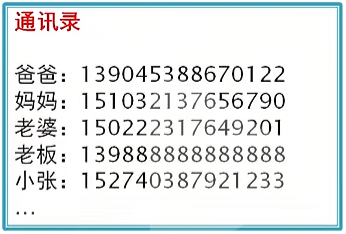
\includegraphics[width=0.8\linewidth]{figures/通讯录.jpeg}
  \caption{生活中的枚举数据：通讯录}
  \label{fig:Contacts}
\end{figure}


电话号码11位数字，按道理来说，一共有 $10^{11}$ 种可能性，
但实际上，我们的通讯录中并不会存入这么多电话号码，
而是只会有其中离散的一部分，比如你亲人
、朋友、同事的号码。此时当我们需要拨打电话时，只能
从通讯录这几个离散的数据里面挑选。

\newpage

枚举的基本规则如\autoref{lst:enum basic}所示


\begin{lstlisting}[language=C,caption={使用 enum 基本规则},label={lst:enum basic}]
enum Color  { RED, GREEN, BLUE };        
// 数值若不自定义，则依次为 0,1,2
enum Weekday{ MON=1, TUE, WED, THU, FRI, SAT, SUN }; 
//若自定义了起始值，则后续依次递增1
enum State { ST_INIT=-5, ST_RUN=8, ST_ERR=9, ST_STOP=100 };
//也可自定义每个枚举值

//注意：枚举数据可以为负数，但必须为整数。
\end{lstlisting}

说完了基本规则，让我们来探讨一下枚举类型变量使用方法，
让我们通过一个示例来加深理解。

\begin{lstlisting}[language=C,caption={使用 enum 定义变量},label={lst:enum var}]
#include <stdio.h>

enum Color { RED, GREEN, BLUE }x;  // 定义枚举类型 Color 并声明变量 x


enum Weekday { MON, TUE, WED, THU, FRI, SAT, SUN };
enum Weekday this_month;  // 声明枚举类型 Weekday 变量 this_month
//这与上面Color的声明方式是等价的。

int main(void) {
    x = RED;  // 给枚举变量 x 赋值  //枚举变量的赋值只能在枚举成员中选择
    this_month = TUE;  // 给枚举变量 this_month 赋值
    printf("Color: %d, Weekday: %d\n", x, this_month);

    return 0;
}
\end{lstlisting}

在上面的示例中，我们定义了两个枚举类型，相信大家已经理解了枚举的
基本用法。接下来我们来接着探讨enum的常量特性。

\texttt{enum}常量是编译期符号，它不同于\texttt{const}常量，也不同于
\texttt{\#define}宏常量在预处理阶段就进行文本替换。
enum常量在编译期被替换为对应的整数值，
不占用任何内存空间，且只能表示整数类型。枚举变量一旦被声明之后
，其值只能在枚举成员中选择，不能赋予其他整数值。这一安全特性使得
枚举常量非常适合表示离散的状态或类别，可以有效提高代码的安全性和可读性。

\end{enumerate}





























\noindent%取消首行缩进
\subsection{命名规则与规范}
\subsubsection{命名规则}
对于字符的组成，变量和常量遵循相同的规则。变量名只能由字母、数字和下划线组成，且首字符不能为
    数字（虽然语法上允许首字符为 \_ ，但在实际编程和标准库约定中有一些潜在风险）
\begin{itemize}
    \item 区分大小写，如 \texttt{age} 与 \texttt{Age} 是不同变量；
    \item 不得与关键字（\texttt{int}, \texttt{return} 等）同名；
\end{itemize}
\subsubsection{代码命名规范}

\begin{enumerate}[label={（\arabic*）}] % 括号编号，使用中文括号编号
  \item 变量命名规范：变量命名通常使用小写字母和下划
  线(例如 \texttt{total\_count})，或者在某些语言中使用驼峰
  式命名。（例如\texttt{totalCount} ）
  \item 常量命名规范:
  常量通常采用全大写字母，单词之间用下划线分
  隔。这是为了让开发者在看到常量时，能够立刻
  识别它们是固定值，而不是可变的数据。
  例如：\texttt{MAX\_SIZE}、\texttt{PI}、\texttt{BUFFER\_LIMIT}。  
\end{enumerate}


  这种约定使得代码更加一致，并且提高了可读性和维护性。


\vspace{1em}%空出一行距离（当前字体高度）
\noindent
\subsection{作用域与生命周期}

\subsubsection{变量}

\begin{enumerate}[label={（\arabic*）}] % 括号编号，使用中文括号编号
  \item 局部变量：定义在函数或语句块中，仅在该范围内有效。每次进入函数时该变量都会被
    重新创建并初始化，生命周期仅限于函数调用期间。当函数或语句块执
    行结束后，变量随即被销毁，内存空间被回收；
  \item 全局变量：定义在所有函数外部，全文件范围内可访问。其生命周
    期从程序开始运行到程序结束，在此期间始终占据固定的内存空间。
    全局变量可被同一文件内的所有函数访问（若需跨文件访问，可使用 extern 声明）。
  \item 静态变量（\texttt{static}）：使用关键字 static 声明。
它的作用域视其属于局部变量还是全局变量而定，但其生命周期贯穿整个程序执行过程。


也就是说，即使该变量为在函数或语句块中定义的局部变量，其在函数调用结束后也不会被销毁，而是保留其上一次的值；
下次进入函数时会继续使用原来的值，而不是重新初始化。
\end{enumerate}
\clearpage


\vspace{1em}%空出一行距离（当前字体高度）
\noindent%取消首行缩进
\textbf{示例}
\begin{lstlisting}[language=C,caption={局部变量与静态局部变量示例},label={lst:foo_static}]
void foo() {
    int x = 0;           // 局部变量
    static int y = 0;    // 静态局部变量
    x++;
    y++;
    printf("x=%d, y=%d\n", x, y);
}
\end{lstlisting}

\vspace{1em}%空出一行距离（当前字体高度）
\vspace{1em}%空出一行距离（当前字体高度）
\vspace{1em}%空出一行距离（当前字体高度）

\noindent
连续调用 \texttt{foo()} 三次的输出为：

\begin{verbatim}
                              x=1, y=1
                              x=1, y=2
                              x=1, y=3
\end{verbatim}



由于局部变量在函数调用时被创建，并在函数结束后自动销毁，因此每次进
入函数时，x 都会重新初始化为 1。而静态局部变量 y 的生命周期贯穿整个
程序运行过程，因此它的值在每次函数调用后都会保留并继续增加。


\subsubsection{常量}

\begin{enumerate}[label={（\arabic*）}] % 括号编号，使用中文括号编号
  \item 局部常量：当常量在函数内部使用 \texttt{const} 声
  明时，它的作用域仅限于该函数或代码块。这样的常量在函数调用结束后被销毁；
  \item 全局常量：当常量在函数内部使用 const 声
  明时，它的作用域仅限于该函数或代码块。这样的常量在函数调用结束后被销毁。
    全局变量可被同一文件内的所有函数访问（若需跨文件访问，可使用 extern 声明）。
  \item 静态常量（\texttt{static}）：与前面静态变量相似，如果常量声明为 static，它
  的生命周期会贯穿整个程序运行期间，即使它的作用域限于声明的文件或函数。
\end{enumerate}






